\documentclass{article}
\usepackage{tabularx}
\usepackage{ctable}
\usepackage[table]{xcolor}
\usepackage{color}
\usepackage{url}
\usepackage{multirow}
\usepackage[utf8x]{inputenc}
\usepackage{fancyvrb}
%\usepackage{llncsdoc}

\begin{document}
\makeatletter
\def\PY@reset{\let\PY@it=\relax \let\PY@bf=\relax%
    \let\PY@ul=\relax \let\PY@tc=\relax%
    \let\PY@bc=\relax \let\PY@ff=\relax}
\def\PY@tok#1{\csname PY@tok@#1\endcsname}
\def\PY@toks#1+{\ifx\relax#1\empty\else%
    \PY@tok{#1}\expandafter\PY@toks\fi}
\def\PY@do#1{\PY@bc{\PY@tc{\PY@ul{%
    \PY@it{\PY@bf{\PY@ff{#1}}}}}}}
\def\PY#1#2{\PY@reset\PY@toks#1+\relax+\PY@do{#2}}

\def\PY@tok@gd{\def\PY@tc##1{\textcolor[rgb]{0.63,0.00,0.00}{##1}}}
\def\PY@tok@gu{\let\PY@bf=\textbf\def\PY@tc##1{\textcolor[rgb]{0.50,0.00,0.50}{##1}}}
\def\PY@tok@gt{\def\PY@tc##1{\textcolor[rgb]{0.00,0.25,0.82}{##1}}}
\def\PY@tok@gs{\let\PY@bf=\textbf}
\def\PY@tok@gr{\def\PY@tc##1{\textcolor[rgb]{1.00,0.00,0.00}{##1}}}
\def\PY@tok@cm{\let\PY@it=\textit\def\PY@tc##1{\textcolor[rgb]{0.25,0.50,0.50}{##1}}}
\def\PY@tok@vg{\def\PY@tc##1{\textcolor[rgb]{0.10,0.09,0.49}{##1}}}
\def\PY@tok@m{\def\PY@tc##1{\textcolor[rgb]{0.40,0.40,0.40}{##1}}}
\def\PY@tok@mh{\def\PY@tc##1{\textcolor[rgb]{0.40,0.40,0.40}{##1}}}
\def\PY@tok@go{\def\PY@tc##1{\textcolor[rgb]{0.50,0.50,0.50}{##1}}}
\def\PY@tok@ge{\let\PY@it=\textit}
\def\PY@tok@vc{\def\PY@tc##1{\textcolor[rgb]{0.10,0.09,0.49}{##1}}}
\def\PY@tok@il{\def\PY@tc##1{\textcolor[rgb]{0.40,0.40,0.40}{##1}}}
\def\PY@tok@cs{\let\PY@it=\textit\def\PY@tc##1{\textcolor[rgb]{0.25,0.50,0.50}{##1}}}
\def\PY@tok@cp{\def\PY@tc##1{\textcolor[rgb]{0.74,0.48,0.00}{##1}}}
\def\PY@tok@gi{\def\PY@tc##1{\textcolor[rgb]{0.00,0.63,0.00}{##1}}}
\def\PY@tok@gh{\let\PY@bf=\textbf\def\PY@tc##1{\textcolor[rgb]{0.00,0.00,0.50}{##1}}}
\def\PY@tok@ni{\let\PY@bf=\textbf\def\PY@tc##1{\textcolor[rgb]{0.60,0.60,0.60}{##1}}}
\def\PY@tok@nl{\def\PY@tc##1{\textcolor[rgb]{0.63,0.63,0.00}{##1}}}
\def\PY@tok@nn{\let\PY@bf=\textbf\def\PY@tc##1{\textcolor[rgb]{0.00,0.00,1.00}{##1}}}
\def\PY@tok@no{\def\PY@tc##1{\textcolor[rgb]{0.53,0.00,0.00}{##1}}}
\def\PY@tok@na{\def\PY@tc##1{\textcolor[rgb]{0.49,0.56,0.16}{##1}}}
\def\PY@tok@nb{\def\PY@tc##1{\textcolor[rgb]{0.00,0.50,0.00}{##1}}}
\def\PY@tok@nc{\let\PY@bf=\textbf\def\PY@tc##1{\textcolor[rgb]{0.00,0.00,1.00}{##1}}}
\def\PY@tok@nd{\def\PY@tc##1{\textcolor[rgb]{0.67,0.13,1.00}{##1}}}
\def\PY@tok@ne{\let\PY@bf=\textbf\def\PY@tc##1{\textcolor[rgb]{0.82,0.25,0.23}{##1}}}
\def\PY@tok@nf{\def\PY@tc##1{\textcolor[rgb]{0.00,0.00,1.00}{##1}}}
\def\PY@tok@si{\let\PY@bf=\textbf\def\PY@tc##1{\textcolor[rgb]{0.73,0.40,0.53}{##1}}}
\def\PY@tok@s2{\def\PY@tc##1{\textcolor[rgb]{0.73,0.13,0.13}{##1}}}
\def\PY@tok@vi{\def\PY@tc##1{\textcolor[rgb]{0.10,0.09,0.49}{##1}}}
\def\PY@tok@nt{\let\PY@bf=\textbf\def\PY@tc##1{\textcolor[rgb]{0.00,0.50,0.00}{##1}}}
\def\PY@tok@nv{\def\PY@tc##1{\textcolor[rgb]{0.10,0.09,0.49}{##1}}}
\def\PY@tok@s1{\def\PY@tc##1{\textcolor[rgb]{0.73,0.13,0.13}{##1}}}
\def\PY@tok@sh{\def\PY@tc##1{\textcolor[rgb]{0.73,0.13,0.13}{##1}}}
\def\PY@tok@sc{\def\PY@tc##1{\textcolor[rgb]{0.73,0.13,0.13}{##1}}}
\def\PY@tok@sx{\def\PY@tc##1{\textcolor[rgb]{0.00,0.50,0.00}{##1}}}
\def\PY@tok@bp{\def\PY@tc##1{\textcolor[rgb]{0.00,0.50,0.00}{##1}}}
\def\PY@tok@c1{\let\PY@it=\textit\def\PY@tc##1{\textcolor[rgb]{0.25,0.50,0.50}{##1}}}
\def\PY@tok@kc{\let\PY@bf=\textbf\def\PY@tc##1{\textcolor[rgb]{0.00,0.50,0.00}{##1}}}
\def\PY@tok@c{\let\PY@it=\textit\def\PY@tc##1{\textcolor[rgb]{0.25,0.50,0.50}{##1}}}
\def\PY@tok@mf{\def\PY@tc##1{\textcolor[rgb]{0.40,0.40,0.40}{##1}}}
\def\PY@tok@err{\def\PY@bc##1{\fcolorbox[rgb]{1.00,0.00,0.00}{1,1,1}{##1}}}
\def\PY@tok@kd{\let\PY@bf=\textbf\def\PY@tc##1{\textcolor[rgb]{0.00,0.50,0.00}{##1}}}
\def\PY@tok@ss{\def\PY@tc##1{\textcolor[rgb]{0.10,0.09,0.49}{##1}}}
\def\PY@tok@sr{\def\PY@tc##1{\textcolor[rgb]{0.73,0.40,0.53}{##1}}}
\def\PY@tok@mo{\def\PY@tc##1{\textcolor[rgb]{0.40,0.40,0.40}{##1}}}
\def\PY@tok@kn{\let\PY@bf=\textbf\def\PY@tc##1{\textcolor[rgb]{0.00,0.50,0.00}{##1}}}
\def\PY@tok@mi{\def\PY@tc##1{\textcolor[rgb]{0.40,0.40,0.40}{##1}}}
\def\PY@tok@gp{\let\PY@bf=\textbf\def\PY@tc##1{\textcolor[rgb]{0.00,0.00,0.50}{##1}}}
\def\PY@tok@o{\def\PY@tc##1{\textcolor[rgb]{0.40,0.40,0.40}{##1}}}
\def\PY@tok@kr{\let\PY@bf=\textbf\def\PY@tc##1{\textcolor[rgb]{0.00,0.50,0.00}{##1}}}
\def\PY@tok@s{\def\PY@tc##1{\textcolor[rgb]{0.73,0.13,0.13}{##1}}}
\def\PY@tok@kp{\def\PY@tc##1{\textcolor[rgb]{0.00,0.50,0.00}{##1}}}
\def\PY@tok@w{\def\PY@tc##1{\textcolor[rgb]{0.73,0.73,0.73}{##1}}}
\def\PY@tok@kt{\def\PY@tc##1{\textcolor[rgb]{0.69,0.00,0.25}{##1}}}
\def\PY@tok@ow{\let\PY@bf=\textbf\def\PY@tc##1{\textcolor[rgb]{0.67,0.13,1.00}{##1}}}
\def\PY@tok@sb{\def\PY@tc##1{\textcolor[rgb]{0.73,0.13,0.13}{##1}}}
\def\PY@tok@k{\let\PY@bf=\textbf\def\PY@tc##1{\textcolor[rgb]{0.00,0.50,0.00}{##1}}}
\def\PY@tok@se{\let\PY@bf=\textbf\def\PY@tc##1{\textcolor[rgb]{0.73,0.40,0.13}{##1}}}
\def\PY@tok@sd{\let\PY@it=\textit\def\PY@tc##1{\textcolor[rgb]{0.73,0.13,0.13}{##1}}}

\def\PYZbs{\char`\\}
\def\PYZus{\char`\_}
\def\PYZob{\char`\{}
\def\PYZcb{\char`\}}
\def\PYZca{\char`\^}
% for compatibility with earlier versions
\def\PYZat{@}
\def\PYZlb{[}
\def\PYZrb{]}
\def\PY@reset{\let\PY@it=\relax \let\PY@bf=\relax%
    \let\PY@ul=\relax \let\PY@tc=\relax%
    \let\PY@bc=\relax \let\PY@ff=\relax}
\def\PY@tok#1{\csname PY@tok@#1\endcsname}
\def\PY@toks#1+{\ifx\relax#1\empty\else%
    \PY@tok{#1}\expandafter\PY@toks\fi}
\def\PY@do#1{\PY@bc{\PY@tc{\PY@ul{%
    \PY@it{\PY@bf{\PY@ff{#1}}}}}}}
\def\PY#1#2{\PY@reset\PY@toks#1+\relax+\PY@do{#2}}

\def\PY@tok@gd{\def\PY@tc##1{\textcolor[rgb]{0.63,0.00,0.00}{##1}}}
\def\PY@tok@gu{\let\PY@bf=\textbf\def\PY@tc##1{\textcolor[rgb]{0.50,0.00,0.50}{##1}}}
\def\PY@tok@gt{\def\PY@tc##1{\textcolor[rgb]{0.00,0.25,0.82}{##1}}}
\def\PY@tok@gs{\let\PY@bf=\textbf}
\def\PY@tok@gr{\def\PY@tc##1{\textcolor[rgb]{1.00,0.00,0.00}{##1}}}
\def\PY@tok@cm{\let\PY@it=\textit\def\PY@tc##1{\textcolor[rgb]{0.25,0.50,0.50}{##1}}}
\def\PY@tok@vg{\def\PY@tc##1{\textcolor[rgb]{0.10,0.09,0.49}{##1}}}
\def\PY@tok@m{\def\PY@tc##1{\textcolor[rgb]{0.40,0.40,0.40}{##1}}}
\def\PY@tok@mh{\def\PY@tc##1{\textcolor[rgb]{0.40,0.40,0.40}{##1}}}
\def\PY@tok@go{\def\PY@tc##1{\textcolor[rgb]{0.50,0.50,0.50}{##1}}}
\def\PY@tok@ge{\let\PY@it=\textit}
\def\PY@tok@vc{\def\PY@tc##1{\textcolor[rgb]{0.10,0.09,0.49}{##1}}}
\def\PY@tok@il{\def\PY@tc##1{\textcolor[rgb]{0.40,0.40,0.40}{##1}}}
\def\PY@tok@cs{\let\PY@it=\textit\def\PY@tc##1{\textcolor[rgb]{0.25,0.50,0.50}{##1}}}
\def\PY@tok@cp{\def\PY@tc##1{\textcolor[rgb]{0.74,0.48,0.00}{##1}}}
\def\PY@tok@gi{\def\PY@tc##1{\textcolor[rgb]{0.00,0.63,0.00}{##1}}}
\def\PY@tok@gh{\let\PY@bf=\textbf\def\PY@tc##1{\textcolor[rgb]{0.00,0.00,0.50}{##1}}}
\def\PY@tok@ni{\let\PY@bf=\textbf\def\PY@tc##1{\textcolor[rgb]{0.60,0.60,0.60}{##1}}}
\def\PY@tok@nl{\def\PY@tc##1{\textcolor[rgb]{0.63,0.63,0.00}{##1}}}
\def\PY@tok@nn{\let\PY@bf=\textbf\def\PY@tc##1{\textcolor[rgb]{0.00,0.00,1.00}{##1}}}
\def\PY@tok@no{\def\PY@tc##1{\textcolor[rgb]{0.53,0.00,0.00}{##1}}}
\def\PY@tok@na{\def\PY@tc##1{\textcolor[rgb]{0.49,0.56,0.16}{##1}}}
\def\PY@tok@nb{\def\PY@tc##1{\textcolor[rgb]{0.00,0.50,0.00}{##1}}}
\def\PY@tok@nc{\let\PY@bf=\textbf\def\PY@tc##1{\textcolor[rgb]{0.00,0.00,1.00}{##1}}}
\def\PY@tok@nd{\def\PY@tc##1{\textcolor[rgb]{0.67,0.13,1.00}{##1}}}
\def\PY@tok@ne{\let\PY@bf=\textbf\def\PY@tc##1{\textcolor[rgb]{0.82,0.25,0.23}{##1}}}
\def\PY@tok@nf{\def\PY@tc##1{\textcolor[rgb]{0.00,0.00,1.00}{##1}}}
\def\PY@tok@si{\let\PY@bf=\textbf\def\PY@tc##1{\textcolor[rgb]{0.73,0.40,0.53}{##1}}}
\def\PY@tok@s2{\def\PY@tc##1{\textcolor[rgb]{0.73,0.13,0.13}{##1}}}
\def\PY@tok@vi{\def\PY@tc##1{\textcolor[rgb]{0.10,0.09,0.49}{##1}}}
\def\PY@tok@nt{\let\PY@bf=\textbf\def\PY@tc##1{\textcolor[rgb]{0.00,0.50,0.00}{##1}}}
\def\PY@tok@nv{\def\PY@tc##1{\textcolor[rgb]{0.10,0.09,0.49}{##1}}}
\def\PY@tok@s1{\def\PY@tc##1{\textcolor[rgb]{0.73,0.13,0.13}{##1}}}
\def\PY@tok@sh{\def\PY@tc##1{\textcolor[rgb]{0.73,0.13,0.13}{##1}}}
\def\PY@tok@sc{\def\PY@tc##1{\textcolor[rgb]{0.73,0.13,0.13}{##1}}}
\def\PY@tok@sx{\def\PY@tc##1{\textcolor[rgb]{0.00,0.50,0.00}{##1}}}
\def\PY@tok@bp{\def\PY@tc##1{\textcolor[rgb]{0.00,0.50,0.00}{##1}}}
\def\PY@tok@c1{\let\PY@it=\textit\def\PY@tc##1{\textcolor[rgb]{0.25,0.50,0.50}{##1}}}
\def\PY@tok@kc{\let\PY@bf=\textbf\def\PY@tc##1{\textcolor[rgb]{0.00,0.50,0.00}{##1}}}
\def\PY@tok@c{\let\PY@it=\textit\def\PY@tc##1{\textcolor[rgb]{0.25,0.50,0.50}{##1}}}
\def\PY@tok@mf{\def\PY@tc##1{\textcolor[rgb]{0.40,0.40,0.40}{##1}}}
\def\PY@tok@err{\def\PY@bc##1{\fcolorbox[rgb]{1.00,0.00,0.00}{1,1,1}{##1}}}
\def\PY@tok@kd{\let\PY@bf=\textbf\def\PY@tc##1{\textcolor[rgb]{0.00,0.50,0.00}{##1}}}
\def\PY@tok@ss{\def\PY@tc##1{\textcolor[rgb]{0.10,0.09,0.49}{##1}}}
\def\PY@tok@sr{\def\PY@tc##1{\textcolor[rgb]{0.73,0.40,0.53}{##1}}}
\def\PY@tok@mo{\def\PY@tc##1{\textcolor[rgb]{0.40,0.40,0.40}{##1}}}
\def\PY@tok@kn{\let\PY@bf=\textbf\def\PY@tc##1{\textcolor[rgb]{0.00,0.50,0.00}{##1}}}
\def\PY@tok@mi{\def\PY@tc##1{\textcolor[rgb]{0.40,0.40,0.40}{##1}}}
\def\PY@tok@gp{\let\PY@bf=\textbf\def\PY@tc##1{\textcolor[rgb]{0.00,0.00,0.50}{##1}}}
\def\PY@tok@o{\def\PY@tc##1{\textcolor[rgb]{0.40,0.40,0.40}{##1}}}
\def\PY@tok@kr{\let\PY@bf=\textbf\def\PY@tc##1{\textcolor[rgb]{0.00,0.50,0.00}{##1}}}
\def\PY@tok@s{\def\PY@tc##1{\textcolor[rgb]{0.73,0.13,0.13}{##1}}}
\def\PY@tok@kp{\def\PY@tc##1{\textcolor[rgb]{0.00,0.50,0.00}{##1}}}
\def\PY@tok@w{\def\PY@tc##1{\textcolor[rgb]{0.73,0.73,0.73}{##1}}}
\def\PY@tok@kt{\def\PY@tc##1{\textcolor[rgb]{0.69,0.00,0.25}{##1}}}
\def\PY@tok@ow{\let\PY@bf=\textbf\def\PY@tc##1{\textcolor[rgb]{0.67,0.13,1.00}{##1}}}
\def\PY@tok@sb{\def\PY@tc##1{\textcolor[rgb]{0.73,0.13,0.13}{##1}}}
\def\PY@tok@k{\let\PY@bf=\textbf\def\PY@tc##1{\textcolor[rgb]{0.00,0.50,0.00}{##1}}}
\def\PY@tok@se{\let\PY@bf=\textbf\def\PY@tc##1{\textcolor[rgb]{0.73,0.40,0.13}{##1}}}
\def\PY@tok@sd{\let\PY@it=\textit\def\PY@tc##1{\textcolor[rgb]{0.73,0.13,0.13}{##1}}}

\def\PYZbs{\char`\\}
\def\PYZus{\char`\_}
\def\PYZob{\char`\{}
\def\PYZcb{\char`\}}
\def\PYZca{\char`\^}
% for compatibility with earlier versions
\def\PYZat{@}
\def\PYZlb{[}
\def\PYZrb{]}
\def\PY@reset{\let\PY@it=\relax \let\PY@bf=\relax%
    \let\PY@ul=\relax \let\PY@tc=\relax%
    \let\PY@bc=\relax \let\PY@ff=\relax}
\def\PY@tok#1{\csname PY@tok@#1\endcsname}
\def\PY@toks#1+{\ifx\relax#1\empty\else%
    \PY@tok{#1}\expandafter\PY@toks\fi}
\def\PY@do#1{\PY@bc{\PY@tc{\PY@ul{%
    \PY@it{\PY@bf{\PY@ff{#1}}}}}}}
\def\PY#1#2{\PY@reset\PY@toks#1+\relax+\PY@do{#2}}

\def\PY@tok@gd{\def\PY@tc##1{\textcolor[rgb]{0.63,0.00,0.00}{##1}}}
\def\PY@tok@gu{\let\PY@bf=\textbf\def\PY@tc##1{\textcolor[rgb]{0.50,0.00,0.50}{##1}}}
\def\PY@tok@gt{\def\PY@tc##1{\textcolor[rgb]{0.00,0.25,0.82}{##1}}}
\def\PY@tok@gs{\let\PY@bf=\textbf}
\def\PY@tok@gr{\def\PY@tc##1{\textcolor[rgb]{1.00,0.00,0.00}{##1}}}
\def\PY@tok@cm{\let\PY@it=\textit\def\PY@tc##1{\textcolor[rgb]{0.25,0.50,0.50}{##1}}}
\def\PY@tok@vg{\def\PY@tc##1{\textcolor[rgb]{0.10,0.09,0.49}{##1}}}
\def\PY@tok@m{\def\PY@tc##1{\textcolor[rgb]{0.40,0.40,0.40}{##1}}}
\def\PY@tok@mh{\def\PY@tc##1{\textcolor[rgb]{0.40,0.40,0.40}{##1}}}
\def\PY@tok@go{\def\PY@tc##1{\textcolor[rgb]{0.50,0.50,0.50}{##1}}}
\def\PY@tok@ge{\let\PY@it=\textit}
\def\PY@tok@vc{\def\PY@tc##1{\textcolor[rgb]{0.10,0.09,0.49}{##1}}}
\def\PY@tok@il{\def\PY@tc##1{\textcolor[rgb]{0.40,0.40,0.40}{##1}}}
\def\PY@tok@cs{\let\PY@it=\textit\def\PY@tc##1{\textcolor[rgb]{0.25,0.50,0.50}{##1}}}
\def\PY@tok@cp{\def\PY@tc##1{\textcolor[rgb]{0.74,0.48,0.00}{##1}}}
\def\PY@tok@gi{\def\PY@tc##1{\textcolor[rgb]{0.00,0.63,0.00}{##1}}}
\def\PY@tok@gh{\let\PY@bf=\textbf\def\PY@tc##1{\textcolor[rgb]{0.00,0.00,0.50}{##1}}}
\def\PY@tok@ni{\let\PY@bf=\textbf\def\PY@tc##1{\textcolor[rgb]{0.60,0.60,0.60}{##1}}}
\def\PY@tok@nl{\def\PY@tc##1{\textcolor[rgb]{0.63,0.63,0.00}{##1}}}
\def\PY@tok@nn{\let\PY@bf=\textbf\def\PY@tc##1{\textcolor[rgb]{0.00,0.00,1.00}{##1}}}
\def\PY@tok@no{\def\PY@tc##1{\textcolor[rgb]{0.53,0.00,0.00}{##1}}}
\def\PY@tok@na{\def\PY@tc##1{\textcolor[rgb]{0.49,0.56,0.16}{##1}}}
\def\PY@tok@nb{\def\PY@tc##1{\textcolor[rgb]{0.00,0.50,0.00}{##1}}}
\def\PY@tok@nc{\let\PY@bf=\textbf\def\PY@tc##1{\textcolor[rgb]{0.00,0.00,1.00}{##1}}}
\def\PY@tok@nd{\def\PY@tc##1{\textcolor[rgb]{0.67,0.13,1.00}{##1}}}
\def\PY@tok@ne{\let\PY@bf=\textbf\def\PY@tc##1{\textcolor[rgb]{0.82,0.25,0.23}{##1}}}
\def\PY@tok@nf{\def\PY@tc##1{\textcolor[rgb]{0.00,0.00,1.00}{##1}}}
\def\PY@tok@si{\let\PY@bf=\textbf\def\PY@tc##1{\textcolor[rgb]{0.73,0.40,0.53}{##1}}}
\def\PY@tok@s2{\def\PY@tc##1{\textcolor[rgb]{0.73,0.13,0.13}{##1}}}
\def\PY@tok@vi{\def\PY@tc##1{\textcolor[rgb]{0.10,0.09,0.49}{##1}}}
\def\PY@tok@nt{\let\PY@bf=\textbf\def\PY@tc##1{\textcolor[rgb]{0.00,0.50,0.00}{##1}}}
\def\PY@tok@nv{\def\PY@tc##1{\textcolor[rgb]{0.10,0.09,0.49}{##1}}}
\def\PY@tok@s1{\def\PY@tc##1{\textcolor[rgb]{0.73,0.13,0.13}{##1}}}
\def\PY@tok@sh{\def\PY@tc##1{\textcolor[rgb]{0.73,0.13,0.13}{##1}}}
\def\PY@tok@sc{\def\PY@tc##1{\textcolor[rgb]{0.73,0.13,0.13}{##1}}}
\def\PY@tok@sx{\def\PY@tc##1{\textcolor[rgb]{0.00,0.50,0.00}{##1}}}
\def\PY@tok@bp{\def\PY@tc##1{\textcolor[rgb]{0.00,0.50,0.00}{##1}}}
\def\PY@tok@c1{\let\PY@it=\textit\def\PY@tc##1{\textcolor[rgb]{0.25,0.50,0.50}{##1}}}
\def\PY@tok@kc{\let\PY@bf=\textbf\def\PY@tc##1{\textcolor[rgb]{0.00,0.50,0.00}{##1}}}
\def\PY@tok@c{\let\PY@it=\textit\def\PY@tc##1{\textcolor[rgb]{0.25,0.50,0.50}{##1}}}
\def\PY@tok@mf{\def\PY@tc##1{\textcolor[rgb]{0.40,0.40,0.40}{##1}}}
\def\PY@tok@err{\def\PY@bc##1{\fcolorbox[rgb]{1.00,0.00,0.00}{1,1,1}{##1}}}
\def\PY@tok@kd{\let\PY@bf=\textbf\def\PY@tc##1{\textcolor[rgb]{0.00,0.50,0.00}{##1}}}
\def\PY@tok@ss{\def\PY@tc##1{\textcolor[rgb]{0.10,0.09,0.49}{##1}}}
\def\PY@tok@sr{\def\PY@tc##1{\textcolor[rgb]{0.73,0.40,0.53}{##1}}}
\def\PY@tok@mo{\def\PY@tc##1{\textcolor[rgb]{0.40,0.40,0.40}{##1}}}
\def\PY@tok@kn{\let\PY@bf=\textbf\def\PY@tc##1{\textcolor[rgb]{0.00,0.50,0.00}{##1}}}
\def\PY@tok@mi{\def\PY@tc##1{\textcolor[rgb]{0.40,0.40,0.40}{##1}}}
\def\PY@tok@gp{\let\PY@bf=\textbf\def\PY@tc##1{\textcolor[rgb]{0.00,0.00,0.50}{##1}}}
\def\PY@tok@o{\def\PY@tc##1{\textcolor[rgb]{0.40,0.40,0.40}{##1}}}
\def\PY@tok@kr{\let\PY@bf=\textbf\def\PY@tc##1{\textcolor[rgb]{0.00,0.50,0.00}{##1}}}
\def\PY@tok@s{\def\PY@tc##1{\textcolor[rgb]{0.73,0.13,0.13}{##1}}}
\def\PY@tok@kp{\def\PY@tc##1{\textcolor[rgb]{0.00,0.50,0.00}{##1}}}
\def\PY@tok@w{\def\PY@tc##1{\textcolor[rgb]{0.73,0.73,0.73}{##1}}}
\def\PY@tok@kt{\def\PY@tc##1{\textcolor[rgb]{0.69,0.00,0.25}{##1}}}
\def\PY@tok@ow{\let\PY@bf=\textbf\def\PY@tc##1{\textcolor[rgb]{0.67,0.13,1.00}{##1}}}
\def\PY@tok@sb{\def\PY@tc##1{\textcolor[rgb]{0.73,0.13,0.13}{##1}}}
\def\PY@tok@k{\let\PY@bf=\textbf\def\PY@tc##1{\textcolor[rgb]{0.00,0.50,0.00}{##1}}}
\def\PY@tok@se{\let\PY@bf=\textbf\def\PY@tc##1{\textcolor[rgb]{0.73,0.40,0.13}{##1}}}
\def\PY@tok@sd{\let\PY@it=\textit\def\PY@tc##1{\textcolor[rgb]{0.73,0.13,0.13}{##1}}}

\def\PYZbs{\char`\\}
\def\PYZus{\char`\_}
\def\PYZob{\char`\{}
\def\PYZcb{\char`\}}
\def\PYZca{\char`\^}
% for compatibility with earlier versions
\def\PYZat{@}
\def\PYZlb{[}
\def\PYZrb{]}
\def\PY@reset{\let\PY@it=\relax \let\PY@bf=\relax%
    \let\PY@ul=\relax \let\PY@tc=\relax%
    \let\PY@bc=\relax \let\PY@ff=\relax}
\def\PY@tok#1{\csname PY@tok@#1\endcsname}
\def\PY@toks#1+{\ifx\relax#1\empty\else%
    \PY@tok{#1}\expandafter\PY@toks\fi}
\def\PY@do#1{\PY@bc{\PY@tc{\PY@ul{%
    \PY@it{\PY@bf{\PY@ff{#1}}}}}}}
\def\PY#1#2{\PY@reset\PY@toks#1+\relax+\PY@do{#2}}

\def\PY@tok@gd{\def\PY@tc##1{\textcolor[rgb]{0.63,0.00,0.00}{##1}}}
\def\PY@tok@gu{\let\PY@bf=\textbf\def\PY@tc##1{\textcolor[rgb]{0.50,0.00,0.50}{##1}}}
\def\PY@tok@gt{\def\PY@tc##1{\textcolor[rgb]{0.00,0.25,0.82}{##1}}}
\def\PY@tok@gs{\let\PY@bf=\textbf}
\def\PY@tok@gr{\def\PY@tc##1{\textcolor[rgb]{1.00,0.00,0.00}{##1}}}
\def\PY@tok@cm{\let\PY@it=\textit\def\PY@tc##1{\textcolor[rgb]{0.25,0.50,0.50}{##1}}}
\def\PY@tok@vg{\def\PY@tc##1{\textcolor[rgb]{0.10,0.09,0.49}{##1}}}
\def\PY@tok@m{\def\PY@tc##1{\textcolor[rgb]{0.40,0.40,0.40}{##1}}}
\def\PY@tok@mh{\def\PY@tc##1{\textcolor[rgb]{0.40,0.40,0.40}{##1}}}
\def\PY@tok@go{\def\PY@tc##1{\textcolor[rgb]{0.50,0.50,0.50}{##1}}}
\def\PY@tok@ge{\let\PY@it=\textit}
\def\PY@tok@vc{\def\PY@tc##1{\textcolor[rgb]{0.10,0.09,0.49}{##1}}}
\def\PY@tok@il{\def\PY@tc##1{\textcolor[rgb]{0.40,0.40,0.40}{##1}}}
\def\PY@tok@cs{\let\PY@it=\textit\def\PY@tc##1{\textcolor[rgb]{0.25,0.50,0.50}{##1}}}
\def\PY@tok@cp{\def\PY@tc##1{\textcolor[rgb]{0.74,0.48,0.00}{##1}}}
\def\PY@tok@gi{\def\PY@tc##1{\textcolor[rgb]{0.00,0.63,0.00}{##1}}}
\def\PY@tok@gh{\let\PY@bf=\textbf\def\PY@tc##1{\textcolor[rgb]{0.00,0.00,0.50}{##1}}}
\def\PY@tok@ni{\let\PY@bf=\textbf\def\PY@tc##1{\textcolor[rgb]{0.60,0.60,0.60}{##1}}}
\def\PY@tok@nl{\def\PY@tc##1{\textcolor[rgb]{0.63,0.63,0.00}{##1}}}
\def\PY@tok@nn{\let\PY@bf=\textbf\def\PY@tc##1{\textcolor[rgb]{0.00,0.00,1.00}{##1}}}
\def\PY@tok@no{\def\PY@tc##1{\textcolor[rgb]{0.53,0.00,0.00}{##1}}}
\def\PY@tok@na{\def\PY@tc##1{\textcolor[rgb]{0.49,0.56,0.16}{##1}}}
\def\PY@tok@nb{\def\PY@tc##1{\textcolor[rgb]{0.00,0.50,0.00}{##1}}}
\def\PY@tok@nc{\let\PY@bf=\textbf\def\PY@tc##1{\textcolor[rgb]{0.00,0.00,1.00}{##1}}}
\def\PY@tok@nd{\def\PY@tc##1{\textcolor[rgb]{0.67,0.13,1.00}{##1}}}
\def\PY@tok@ne{\let\PY@bf=\textbf\def\PY@tc##1{\textcolor[rgb]{0.82,0.25,0.23}{##1}}}
\def\PY@tok@nf{\def\PY@tc##1{\textcolor[rgb]{0.00,0.00,1.00}{##1}}}
\def\PY@tok@si{\let\PY@bf=\textbf\def\PY@tc##1{\textcolor[rgb]{0.73,0.40,0.53}{##1}}}
\def\PY@tok@s2{\def\PY@tc##1{\textcolor[rgb]{0.73,0.13,0.13}{##1}}}
\def\PY@tok@vi{\def\PY@tc##1{\textcolor[rgb]{0.10,0.09,0.49}{##1}}}
\def\PY@tok@nt{\let\PY@bf=\textbf\def\PY@tc##1{\textcolor[rgb]{0.00,0.50,0.00}{##1}}}
\def\PY@tok@nv{\def\PY@tc##1{\textcolor[rgb]{0.10,0.09,0.49}{##1}}}
\def\PY@tok@s1{\def\PY@tc##1{\textcolor[rgb]{0.73,0.13,0.13}{##1}}}
\def\PY@tok@sh{\def\PY@tc##1{\textcolor[rgb]{0.73,0.13,0.13}{##1}}}
\def\PY@tok@sc{\def\PY@tc##1{\textcolor[rgb]{0.73,0.13,0.13}{##1}}}
\def\PY@tok@sx{\def\PY@tc##1{\textcolor[rgb]{0.00,0.50,0.00}{##1}}}
\def\PY@tok@bp{\def\PY@tc##1{\textcolor[rgb]{0.00,0.50,0.00}{##1}}}
\def\PY@tok@c1{\let\PY@it=\textit\def\PY@tc##1{\textcolor[rgb]{0.25,0.50,0.50}{##1}}}
\def\PY@tok@kc{\let\PY@bf=\textbf\def\PY@tc##1{\textcolor[rgb]{0.00,0.50,0.00}{##1}}}
\def\PY@tok@c{\let\PY@it=\textit\def\PY@tc##1{\textcolor[rgb]{0.25,0.50,0.50}{##1}}}
\def\PY@tok@mf{\def\PY@tc##1{\textcolor[rgb]{0.40,0.40,0.40}{##1}}}
\def\PY@tok@err{\def\PY@bc##1{\fcolorbox[rgb]{1.00,0.00,0.00}{1,1,1}{##1}}}
\def\PY@tok@kd{\let\PY@bf=\textbf\def\PY@tc##1{\textcolor[rgb]{0.00,0.50,0.00}{##1}}}
\def\PY@tok@ss{\def\PY@tc##1{\textcolor[rgb]{0.10,0.09,0.49}{##1}}}
\def\PY@tok@sr{\def\PY@tc##1{\textcolor[rgb]{0.73,0.40,0.53}{##1}}}
\def\PY@tok@mo{\def\PY@tc##1{\textcolor[rgb]{0.40,0.40,0.40}{##1}}}
\def\PY@tok@kn{\let\PY@bf=\textbf\def\PY@tc##1{\textcolor[rgb]{0.00,0.50,0.00}{##1}}}
\def\PY@tok@mi{\def\PY@tc##1{\textcolor[rgb]{0.40,0.40,0.40}{##1}}}
\def\PY@tok@gp{\let\PY@bf=\textbf\def\PY@tc##1{\textcolor[rgb]{0.00,0.00,0.50}{##1}}}
\def\PY@tok@o{\def\PY@tc##1{\textcolor[rgb]{0.40,0.40,0.40}{##1}}}
\def\PY@tok@kr{\let\PY@bf=\textbf\def\PY@tc##1{\textcolor[rgb]{0.00,0.50,0.00}{##1}}}
\def\PY@tok@s{\def\PY@tc##1{\textcolor[rgb]{0.73,0.13,0.13}{##1}}}
\def\PY@tok@kp{\def\PY@tc##1{\textcolor[rgb]{0.00,0.50,0.00}{##1}}}
\def\PY@tok@w{\def\PY@tc##1{\textcolor[rgb]{0.73,0.73,0.73}{##1}}}
\def\PY@tok@kt{\def\PY@tc##1{\textcolor[rgb]{0.69,0.00,0.25}{##1}}}
\def\PY@tok@ow{\let\PY@bf=\textbf\def\PY@tc##1{\textcolor[rgb]{0.67,0.13,1.00}{##1}}}
\def\PY@tok@sb{\def\PY@tc##1{\textcolor[rgb]{0.73,0.13,0.13}{##1}}}
\def\PY@tok@k{\let\PY@bf=\textbf\def\PY@tc##1{\textcolor[rgb]{0.00,0.50,0.00}{##1}}}
\def\PY@tok@se{\let\PY@bf=\textbf\def\PY@tc##1{\textcolor[rgb]{0.73,0.40,0.13}{##1}}}
\def\PY@tok@sd{\let\PY@it=\textit\def\PY@tc##1{\textcolor[rgb]{0.73,0.13,0.13}{##1}}}

\def\PYZbs{\char`\\}
\def\PYZus{\char`\_}
\def\PYZob{\char`\{}
\def\PYZcb{\char`\}}
\def\PYZca{\char`\^}
% for compatibility with earlier versions
\def\PYZat{@}
\def\PYZlb{[}
\def\PYZrb{]}
\makeatother

\title{Scalable applications in a distributed environment}
\author{Simon Norberg - norberg.simon@gmail.com\\
        Filip Andersson - flpandersson@gmail.com }
%\institute{Blekinge Institute of Technology}
\date{\today}
\maketitle

\newpage
%fixme: Make this look better
\begin{flushright}
\large{\emph{It is not the strongest of the species that survives, nor the most 
intelligent that survives. It is the one that is the most adaptable to change.}
\newline
\emph{- -Charles Darwin (1809-1882)}}
\end{flushright}
\newpage
 
%\begin{abstract}
%TODO
%\end{abstract}
 
\section{Introduction}

Distribution and scalability is becoming an important issue in todays
application development \cite{rellermeyer2007services}.
The need for an application to scale between a few users up to several millions 
on very short notice gives developers limited time to modify and/or redesign 
the application, so having an already scalable system has a lot of benefits. 
If a system looses its ability to scale, and thereby cannot support more users, 
it may quickly loose its target audience to a competitor. Furthermore, being able 
to modify and update parts of the system separately, rather than everything at 
once, makes application maintenance significantly easier and downtime minimal 
in production systems.

\subsection{Background}

A scalable system is a system that is flexible and adaptive to changing
conditions, such as an increase in system load, new system components etc., and
that can be economically deployed in many configurations, small as well as
large \cite{jogalekar2000evaluating}. The scalability of a system depends on
how well it can exploit functional modularity, structural regularity and
hierarchy \cite{lipson2007principles}.

To make a system modular it can be implemented using \emph{OSGi} and
\emph{R-OSGi} \cite{rellermeyer2007services} \cite{marples2001open}. By using these frameworks one can
update and add components to ones system at will, and manage different
components without having to bring down the entire system. When deployed,
R-OSGi can be used to turn the application into a distributed application by
indicating where the different modules should be deployed
\cite{rellermeyer2007r}, which can be used to greatly simplify development of
distributed systems.

\emph{Distributed Computing}, perhaps more known as \emph{Cloud Computing}, is becoming a
more and more common approach to software development. The basic concept of
distributed computing is to make different services available in the so called
'cloud', which means that these services are reachable from anywhere one has
internet access. These services can, for example, be things like e-mail,
document editing, social networks and much more. The fact that these services
are so widely distributed places high demands on the number of users that can
be supported. These demands can be accommodated by simply making sure the
systems have a large amount of resources from the start, or adding resources
from time to time. However, if there's less users on the system than it has
capacity for, this approach quickly becomes expensive due to a lot of unused
resources. This problem can be solved by making the system scalable, i.e. that
it uses resources in proportion to the number of current users. If the user
base drops, it will use less resources, and when more people are using the
system it will use more. By making a system scalable, one makes it able to
adapt to changing conditions and environments, which is important since a
system is generally developed to run over a relatively large period of time,
during which a lot of things may rapidly change \cite{van1998software}
\cite{caruso1997toward}. This can be crucial to, among other things, reduce
software development cost \cite{fayad2005towards}.

To promote scalability in a distributed setting one can use, for example, the
\emph{Message Passing Interface (MPI)} which enables message passing between
parallel programs running on computer clusters. MPI is
an well tested and de facto standard for writing scalable software in any
language and on any platform. MPI makes it easy to delegate work in an
scalable and distributed environment and at the same time collect the results
form different nodes. MPI also allows an arbitrary number of nodes in the 
system with make it easy to add more resources when performance needs to
be improved. \cite{gropp1996high}
 
\subsection{Goals} 

What we intend to investigate is what needs to be considered
when developing a scalable distributed system, and to what cost these features
comes at. We believe that while the cost of these features may initially be
higher, the cost of maintainability is lower. We hope that the outcome of our
research will be useful for people trying to determine whether or not to strive
towards implementing a scalable distributed system from the start, rather than
incrementally increasing system capacity during the system's lifetime.

\newpage

\section{Research questions}

\begin{itemize}
\item{RQ1: How do one successfully develop a scalable distributed system? Which
factors needs to be considered, and how does one achieve these? Without knowing
what needs to be done, developing a high-grade scalable system may be
difficult, and cost a lot of extra time.} 

\item{RQ1.1: Which technologies, libraries and software can one use to achieve
high-grade scalability? Not all technologies etc. support a high level of
scalability, and knowing the difference between the ones who do and the ones
who do not can save a lot of expenses.}

\item{RQ2: Which extra costs do the development of scalable systems lead to?} 
\item{RQ2.1: When done in advance?} 
\item{RQ2.2: When done after the initial development?} 

\item{RQ3: Which kind of systems can benefit from having high-grade scalability?
It is important to know if a certain system actually benefits from being highly
scalable, and if so, how much. If the benefits are relatively small, there 
might be cheaper ways of developing it.}


\end{itemize}

\section{Research methodology}

We will be using a Literature Review and a Post-mortem analysis to conduct our 
research. 

\subsection{Literature review design}

We will be searching for literature for our review mainly on Google Scholar and
on BTH's article database Elin. The keywords we will be using while searching 
will be focused on terms related to distributed systems and scalability.

The research started with the keywords scalable and distributed systems,
from there we read article that looked promising first by just looking on
the topic and if it looked relevant for our thesis, we took a closer look
at the abstract. After reading the abstract we made a decision if the paper
was in the scope of our project and if it was that we selected it. And used
terminology found in that paper to find further papers on which the same 
process was used. 
\newline

List of keywords:
\begin{itemize}
\item{scalable systems (Google Scholar)}
\item{python parallel (Google Scholar)}
\item{mpi (Google Scholar)}
\item{Distributed systems AND scalable design (ELIN)}
\item{Distributed environments services osgi (ELIN)}
\item{Scalable distribution AND software (ELIN)}
\item{Scalable development AND cost (ELIN)}
\item{Scalability AND distributed systems (ELIN)}
\item{Distributed Applications AND Software Modularization (ELIN)}
\end{itemize}

\subsection{Post-mortem analysis design}

\subsubsection{MPI}
We will study a classical and well tested approach to writing
scalable distributed systems with MPI \cite{gropp1996high}. MPI have easy
to use python bindings \cite{miller2002pympi} \cite{millerparallel} we will be
using to write test programs that test the capabilities of MPI and compare the
performance and cost to develop.
We will be measuring:
\begin{itemize}
\item Time to develop
\begin{itemize}
\item{ \textbf{Why} - If we know how much time it takes to develop a scalable application with
MPI we can measure the cost of developing the scalable application. Which is needed to
know in which cases it may be cost efficient.}
\item{ \textbf{How} - By keeping track of spent time for writing the software, 
and also by doing it more than one time we can see how much time is saved
when you starts to get used to MPI.}
\end{itemize}
\item Lines of code
\begin{itemize}
\item{ \textbf{Why} - The easiest metric of how complex and hard to write and
 maintain a program is. The metric is a bit problematic if you compare
 code written by different programmers, some write short and hard to read
 code and other more verbose but easier to read. But by letting the same
 programmers write both of the applications we hope to overcome that 
 difference.}
\item{ \textbf{How} - Count number of lines with \emph{wc -l}}
\end{itemize}
\item How easy the code is to understand
\begin{itemize}
\item{ \textbf{Why} - Code that is easy to understand is also easy to maintain and extend. }
\item{ \textbf{How} - Hard to objectively measure, but we will compare how much harder/easier we 
 feel it is to understand the MPI code. }
\end{itemize}
\item How easy it is to extend the program
\begin{itemize}
\item{ \textbf{Why} - If the application becomes harder to extend and improve upon 
when using MPI it maybe isn't feasible to write applications that
needs to be extended further on with MPI.}
\item{ \textbf{How} - Measure how much work it takes to extend the application with 
		some example feature}
\end{itemize}
\item Performance - How fast do the application run
\begin{itemize}
\item{ \textbf{Why} - Because one of the main reason for scalability is to increase the
 performance we want to know how much we are able to increase it by using MPI. }
\item{ \textbf{How} - Measure the time to run the program with \emph{time}}
\end{itemize}
\item Scalability - how well do it scale when adding more resources
\begin{itemize}
\item{ \textbf{Why} - Optimal we would like to have an application that scales linear
 so when doubling the resources the performance also doubles. This is probably 
 not the case, but we want to know how much performance gain we get by adding
 more resources to the system. }
\item{ \textbf{How} - Adding more resource to the system and then measure performance
 again}
\end{itemize}
\item Performance when using only one node, e.g. overhead for MPI
\begin{itemize}
\item{ \textbf{Why} - We want to know how much performance penalty we get for using
MPI in a system that do not need the scalability of MPI, either because it is 
less usage at the time (e.g. due to it being night) or because the system
don't have a high usage yet and maybe never will.}
\item{ \textbf{How} - Setting up MPI with just one node and measure the performance
 compared to the non scalable application. }
\end{itemize}
\end{itemize}


\section{Post mortem results}
\subsection{Pre study}
We started by look at the different MPI bindings provided for python, the result
was overwhelming and we found several different bindings providing the same
functionality. After some research we chose to use boost-mpi python bindings
\cite{boost-mpi}. This bindings locked well maintained and had a proper
debian package and had example code that worked out of the box, as opposed to
the other bindings we tested. The problem was probably that it existed more
than one library with the exact same name but was used differently and it was
hard to know what library different examples was supposed to work with. 

\subsection{Problem}
Before we could write a scalable application we had to choose what problem we
wanted to solve with our application; we chose to write an application that
would try to find what password a user had from the hash it generated.
The reason is that it requires a lot of cpu time to calculate and it is 
very easy to split up in several parts and doing them parallel.

\subsection{Solution}
The solutions works by iterating over a dictionary off $\sim$3.6 Million words
and test if the word matches the supplied hash and also check if word followed
by a digit match. The reason that we also check the word followed by a digit
is to increase the load on the system due to the execution time being to 
low to reliable measure and reproduce the data when only hashing $\sim$3.6
Million words.

\subsection{Set up}
2 Computers with:
\begin{itemize}
\item Intel(R) Core 2 Duo CPU6600  @ 2.40GHz
\item 2 GB Memory
\item Local 1 Gbit lan
\item Debian Squeeze
\item mpich 1.2.7-9.1
\item boost-mpi-python 1.42.0
\item Our test application \cite{pympi-test}
\end{itemize}

\subsection{Measuring}
Measuring was done by running the application 10 times for every number of
instances between 1 and 10 and then calculating the mean time for each 
number of instances. A non parallel program was also written and used to
compare to our parallel application.

\subsection{Scalability}
This table and diagram shows how much performance is increased for every
new instance of MPI stared.

\rowcolors{1}{gray!40}{}
\begin{tabular}{c c c}
  \rowcolor[gray]{0.5}
  {\bf Instances} & {\bf python MPI (sec)} & {\bf Linear Scalability (sec)} \\
  1 & 101,48 & 101,48 \\
  2 & 53,66  & 50,74  \\
  3 & 36,03  & 33,83  \\
  4 & 28,37  & 25,37  \\
  5 & 34,24  & 25,37  \\
  6 & 29,32  & 25,37  \\
  7 & 31,57  & 25,37  \\
  8 & 29,67  & 25,37  \\
  9 & 31,73  & 25,37  \\
 10 & 29,94  & 25,37  \\
\rowcolor[gray]{0.5}
\end{tabular}
\rowcolors{1}{gray!0}{}

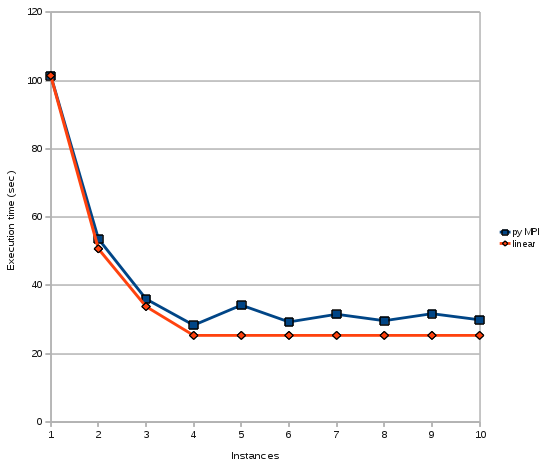
\includegraphics[width=\textwidth]{img/scalabilty-pympi.png}
\\\small{ Total number of cores in the system was 4, so performance stopped
increasing when adding more instances than 4. }

We can see that the performance almost increase linear when adding more
resource to the system. This shows that our application don't have any
major bottlenecks and it would be easy to increase the performance
of the application by just adding more resource when its needed.

\subsection{Scalable vs. Non Scalable Systems}
This table and diagrams compare our scalable application towards an non
scalable application

\rowcolors{1}{gray!40}{}
\begin{tabular}{c c c}
  \rowcolor[gray]{0.5}
  {\bf Instances} & {\bf python MPI (sec)} & {\bf Non Scalable System (sec)} \\
  1 & 101,48 & 96.82 \\
  2 & 53,66  & 96.82  \\
  3 & 36,03  & 96.82  \\
  4 & 28,37  & 96.82  \\
  5 & 34,24  & 96.82  \\
  6 & 29,32  & 96.82  \\
  7 & 31,57  & 96.82  \\
  8 & 29,67  & 96.82  \\
  9 & 31,73  & 96.82  \\
 10 & 29,94  & 96.82  \\
\rowcolor[gray]{0.5}
\end{tabular}
\rowcolors{1}{gray!0}{}
\newline
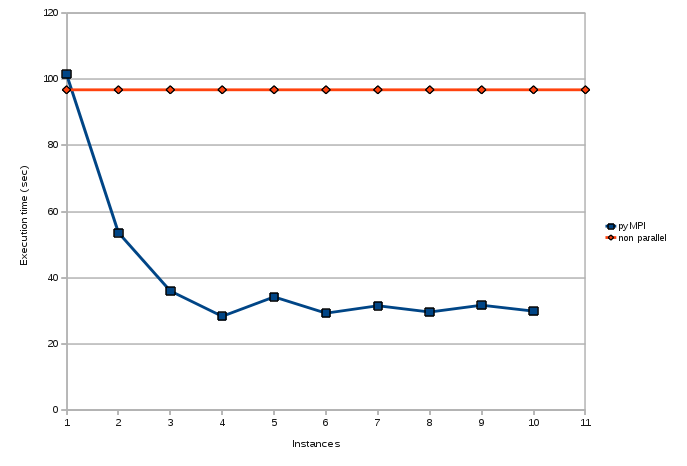
\includegraphics[width=\textwidth]{img/parallel-vs-non-parallel.png}

From this we can see that we have a small performance loss (5\%) due the usage
of MPI but if we have more than one core to run on we get drastically better
performance.


\subsection{Complexity}
We have measured the complexity of both our parallel and non parallel
application, and presents the results below.

\rowcolors{1}{gray!40}{}
\begin{tabular}{l c c}
  \rowcolor[gray]{0.5}
  {\bf Measurement} & {\bf python MPI} & {\bf Non Scalable System} \\
  Lines of code &  23  &  21 \\
  Block Depth   &   5  &   5  \\
  Blocks        &   9  &   9  \\
  Tokens        & 267  & 242  \\
  McCabe Complexity\cite{mccabe1976complexity} \_\_main\_\_ & 2  & 2 \\
  McCabe Complexity\cite{mccabe1976complexity} find\_password & 7  & 7  \\
\rowcolor[gray]{0.5}
\end{tabular}
\rowcolors{1}{gray!0}{}
\\\small{ Measurements done with pyMetrics\cite{pymetrics}}

From  

\paragraph{Parallel version of the application}
\begin{Verbatim}[commandchars=\\\{\}]
\PY{k+kn}{import} \PY{n+nn}{random}\PY{o}{,} \PY{n+nn}{hashlib}
\PY{k+kn}{from} \PY{n+nn}{boost} \PY{k+kn}{import} \PY{n}{mpi}
\PY{k+kn}{from} \PY{n+nn}{glob} \PY{k+kn}{import} \PY{n}{glob}

\PY{k}{def} \PY{n+nf}{find\PYZus{}password}\PY{p}{(}\PY{n}{brute\PYZus{}hash}\PY{p}{,} \PY{n}{start\PYZus{}chunk}\PY{p}{,} \PY{n}{nr\PYZus{}of\PYZus{}instances}\PY{p}{)}\PY{p}{:}
	\PY{n}{files} \PY{o}{=} \PY{n}{glob}\PY{p}{(}\PY{l+s}{"}\PY{l+s}{pympi-test/dicts/x*}\PY{l+s}{"}\PY{p}{)}
	\PY{k}{for} \PY{n}{i} \PY{o+ow}{in} \PY{n+nb}{range}\PY{p}{(}\PY{n}{start\PYZus{}chunk}\PY{p}{,} \PY{n+nb}{len}\PY{p}{(}\PY{n}{files}\PY{p}{)}\PY{p}{,} \PY{n}{nr\PYZus{}of\PYZus{}instances}\PY{p}{)}\PY{p}{:} 
		\PY{n}{words} \PY{o}{=} \PY{n+nb}{open}\PY{p}{(}\PY{n}{files}\PY{p}{[}\PY{n}{i}\PY{p}{]}\PY{p}{)}
		\PY{k}{for} \PY{n}{word} \PY{o+ow}{in} \PY{n}{words}\PY{o}{.}\PY{n}{readlines}\PY{p}{(}\PY{p}{)}\PY{p}{:}
			\PY{k}{for} \PY{n}{i} \PY{o+ow}{in} \PY{n+nb}{range}\PY{p}{(}\PY{o}{-}\PY{l+m+mi}{1}\PY{p}{,}\PY{l+m+mi}{10}\PY{p}{)}\PY{p}{:}
				\PY{k}{if} \PY{n}{i} \PY{o}{==} \PY{o}{-}\PY{l+m+mi}{1}\PY{p}{:}
					\PY{n}{hash\PYZus{}word} \PY{o}{=} \PY{n}{word}\PY{o}{.}\PY{n}{strip}\PY{p}{(}\PY{p}{)}
				\PY{k}{else}\PY{p}{:}
					\PY{n}{hash\PYZus{}word} \PY{o}{=} \PY{n}{word}\PY{o}{.}\PY{n}{strip}\PY{p}{(}\PY{p}{)} \PY{o}{+} \PY{n+nb}{str}\PY{p}{(}\PY{n}{i}\PY{p}{)}
				\PY{n}{new\PYZus{}hash} \PY{o}{=} \PY{n}{hashlib}\PY{o}{.}\PY{n}{sha256}\PY{p}{(}\PY{n}{hash\PYZus{}word}\PY{p}{)}\PY{o}{.}\PY{n}{hexdigest}\PY{p}{(}\PY{p}{)}
				\PY{k}{if} \PY{n}{new\PYZus{}hash} \PY{o}{==} \PY{n}{brute\PYZus{}hash}\PY{p}{:}
					\PY{k}{return} \PY{n}{hash\PYZus{}word}
	\PY{k}{return} \PY{n+nb+bp}{None}

\PY{k}{if} \PY{n}{\PYZus{}\PYZus{}name\PYZus{}\PYZus{}}\PY{o}{==}\PY{l+s}{"}\PY{l+s}{\PYZus{}\PYZus{}main\PYZus{}\PYZus{}}\PY{l+s}{"}\PY{p}{:}
	\PY{n}{rank}\PY{p}{,} \PY{n}{size} \PY{o}{=} \PY{n}{mpi}\PY{o}{.}\PY{n}{rank}\PY{p}{,} \PY{n}{mpi}\PY{o}{.}\PY{n}{size}
	\PY{n}{passwd} \PY{o}{=} \PY{n}{find\PYZus{}password}\PY{p}{(}\PY{n}{hashlib}\PY{o}{.}\PY{n}{sha256}\PY{p}{(}\PY{l+s}{"}\PY{l+s}{simon22}\PY{l+s}{"}\PY{p}{)}\PY{o}{.}\PY{n}{hexdigest}\PY{p}{(}\PY{p}{)}\PY{p}{,} \PY{n}{rank}\PY{p}{,} \PY{n}{size}\PY{p}{)}
	\PY{k}{print} \PY{n}{passwd}
\end{Verbatim}

\paragraph{Non Parallel version of the application}
\begin{Verbatim}[commandchars=\\\{\}]
\PY{k+kn}{import} \PY{n+nn}{random}\PY{o}{,} \PY{n+nn}{hashlib}
\PY{k+kn}{from} \PY{n+nn}{glob} \PY{k+kn}{import} \PY{n}{glob}

\PY{k}{def} \PY{n+nf}{find\PYZus{}password}\PY{p}{(}\PY{n}{brute\PYZus{}hash}\PY{p}{,} \PY{n}{start\PYZus{}chunk}\PY{p}{,} \PY{n}{nr\PYZus{}of\PYZus{}instances}\PY{p}{)}\PY{p}{:}
	\PY{n}{files} \PY{o}{=} \PY{n}{glob}\PY{p}{(}\PY{l+s}{"}\PY{l+s}{pympi-test/dicts/x*}\PY{l+s}{"}\PY{p}{)}
	\PY{k}{for} \PY{n}{i} \PY{o+ow}{in} \PY{n+nb}{range}\PY{p}{(}\PY{n}{start\PYZus{}chunk}\PY{p}{,} \PY{n+nb}{len}\PY{p}{(}\PY{n}{files}\PY{p}{)}\PY{p}{,} \PY{n}{nr\PYZus{}of\PYZus{}instances}\PY{p}{)}\PY{p}{:} 
		\PY{n}{words} \PY{o}{=} \PY{n+nb}{open}\PY{p}{(}\PY{n}{files}\PY{p}{[}\PY{n}{i}\PY{p}{]}\PY{p}{)}
		\PY{k}{for} \PY{n}{word} \PY{o+ow}{in} \PY{n}{words}\PY{o}{.}\PY{n}{readlines}\PY{p}{(}\PY{p}{)}\PY{p}{:}
			\PY{k}{for} \PY{n}{i} \PY{o+ow}{in} \PY{n+nb}{range}\PY{p}{(}\PY{o}{-}\PY{l+m+mi}{1}\PY{p}{,}\PY{l+m+mi}{10}\PY{p}{)}\PY{p}{:}
				\PY{k}{if} \PY{n}{i} \PY{o}{==} \PY{o}{-}\PY{l+m+mi}{1}\PY{p}{:}
					\PY{n}{hash\PYZus{}word} \PY{o}{=} \PY{n}{word}\PY{o}{.}\PY{n}{strip}\PY{p}{(}\PY{p}{)}
				\PY{k}{else}\PY{p}{:}
					\PY{n}{hash\PYZus{}word} \PY{o}{=} \PY{n}{word}\PY{o}{.}\PY{n}{strip}\PY{p}{(}\PY{p}{)} \PY{o}{+} \PY{n+nb}{str}\PY{p}{(}\PY{n}{i}\PY{p}{)}
				\PY{n}{new\PYZus{}hash} \PY{o}{=} \PY{n}{hashlib}\PY{o}{.}\PY{n}{sha256}\PY{p}{(}\PY{n}{hash\PYZus{}word}\PY{p}{)}\PY{o}{.}\PY{n}{hexdigest}\PY{p}{(}\PY{p}{)}
				\PY{k}{if} \PY{n}{new\PYZus{}hash} \PY{o}{==} \PY{n}{brute\PYZus{}hash}\PY{p}{:}
					\PY{k}{return} \PY{n}{hash\PYZus{}word}
	\PY{k}{return} \PY{n+nb+bp}{None}

\PY{k}{if} \PY{n}{\PYZus{}\PYZus{}name\PYZus{}\PYZus{}}\PY{o}{==}\PY{l+s}{"}\PY{l+s}{\PYZus{}\PYZus{}main\PYZus{}\PYZus{}}\PY{l+s}{"}\PY{p}{:}
	\PY{n}{passwd} \PY{o}{=} \PY{n}{find\PYZus{}password}\PY{p}{(}\PY{n}{hashlib}\PY{o}{.}\PY{n}{sha256}\PY{p}{(}\PY{l+s}{"}\PY{l+s}{simon22}\PY{l+s}{"}\PY{p}{)}\PY{o}{.}\PY{n}{hexdigest}\PY{p}{(}\PY{p}{)}\PY{p}{,} \PY{l+m+mi}{0}\PY{p}{,} \PY{l+m+mi}{1}\PY{p}{)}
	\PY{k}{print} \PY{n}{passwd}
\end{Verbatim}

 
\section{Literature study results}

\subsection{Initial search results}
When we applied our search strings for the literature study we found the
following articles:

(See list of references)

\subsection{Selected papers}
During the process of reviewing the found papers we removed three that we felt
did not, while being relevant, contribute to our cause, and thus they were
removed. 

The ones we selected are mentioned here:

\paragraph{Evaluating the scalability of distributed systems}
\cite{jogalekar2000evaluating}

\emph{A system design is scalable if it can be economically deployed at a range
of scales, in both small and large con- figurations. Little attention has been
paid to measuring and comparing the scalability of different designs of
software for distributed operation. Recently a new measure of scal- ability
(called here P-scalability since it based on the “power” metric) has been
defined specifically for distributed systems. This paper generalizes the
metric, defines a scaling path embodying a strategy modifying the system as it
is scaled up, and employs scalability enabling parameters which adapt the
system to give the maximum value of the scalability metric, at any point along
the scaling path.}

\paragraph{Principles of modularity, regularity and hierarchy for scalable
systems} \cite{lipson2007principles}

\emph{Scalability of open-ended evolutionary processes depends on their ability
to exploit functional modularity, structural regularity and hierarchy.  This
paper offers a number of observations about properties, dependencies and
tradeoffs among these principles and proposes a formal model where such ele-
ments can be examined.}

\paragraph{Software engineering for the scalable distributed applications}
\cite{van1998software}

\emph{A major problem in the development of distributed applications is that
one cannot assume that the environment in which the application is to operate
will remain the same. This means that developers must take into account that
the application should be easy to adapt, A requirement that is often formulated
imprecisely is that an application should be scalable. The authors concentrate
on scalability as a requirement for distributed applications, what it actually
means, and how it can be taken into account during system design and
implementation. They present a framework in which scalability requirements can
be formulated precisely. In addition, they present an approach by which
scalability can be taken into account during application development. Their
approach consists of an engineering method for distributing functionality,
combined with an object-based implementation framework for applying scaling
techniques such as replication and caching.}

\paragraph{Toward a scalable design for command and control systems}
\cite{caruso1997toward}

\emph{ Command and control systems exist in a world of con- stantly shifing
demands and expectations: therefore, pro- ducing scalable, evolvable systems
has always been a priority of system designers. Howevel; the need to meet
peiformance requirements has ofen been a restraint on scalability goals.
Advances in the speed and capacity of computational and communications
equipment have sub- stantially increased the range of scalability that can be
achieved while still meeting performunce requirements.  The High Performance
Distributed Computing Program (HiPer-D) has demonstrated a design for the AEGIS
weapons system, which is close to achieving the full range of operational
requirements while providing scalability along several dimensions. This paper
discusses the HiPer-D design, its context, development, and efforts to achieve
system level performance.}

\paragraph{Towards Scalable and Adaptable Software Architectures} \cite{fayad2005towards}

\emph{Developing scalable and adaptable architectures that can accommodate
evolving changes is crucial for reducing software development cost. To achieve
scalability and adaptability, developers should be able to identify where and
how new (current) layers will be added (removed) from the architecture.
Failing to do so may lead to software architectures that require a considerable
modifications when the system evolves or changes due to new or added
requirements. In this paper, we address the problem of developing scalable
software architectures that can accommodate new and/or modified requirements
without the need for re-developing the architecture from scratch. The approach
is demonstrated through a case study.}

\paragraph{A high-performance, portable implementation of the MPI message passing
interface standard} \cite{gropp1996high}

\emph{MPI (Message Passing Interface) is a specification for a standard library
for message passing that was defined by the MPI Forum, a broadly based group of
parallel computer vendors, library writers, and applications specialists.
Multiple implementations of MPI have been developed. In this paper, we describe
MPICH, unique among existing implementations in its design goal of combining
portability with high performance. We document its portability and performance
and describe the architecture by which these features are simultaneously
achieved. We also discuss the set of tools that accompany the free distribution
of MPICH, which constitute the beginnings of a portable parallel programming
environment. A project of this scope inevitably imparts lessons about parallel
computing, the specification being followed, the current hardware and software
environment for parallel computing, and project management; we describe those
we have learned.  Finally, we discuss future developments for MPICH, including
those necessary to accommodate extensions to the MPI Standard now being
contemplated by the MPI Forum.}

\paragraph{pyMPI - An introduction to parallel Python using MPI}
\cite{miller2002pympi}

\emph{The interpreted language, Python, provides a good framework for building
scripts and control frameworks. While Python has a (co-routining) thread model,
its basic design is not particularly appropriate for parallel programming. The
pyMPI extension set is designed to provide parallel operations for Python on
distributed, parallel machines using MPI.}

\paragraph{Parallel, distributed scripting with python} \cite{millerparallel}

\emph{Parallel computers used to be, for the most part, one-of-a-kind systems
which were extremely difficult to program portably. With SMP architectures, the
advent of the POSIX thread API and OpenMP gave developers ways to portably
exploit on-the-box shared memory parallelism. Since these architectures
didn't scale cost-effectively, distributed memory clusters were developed. The
associated MPI message passing libraries gave these systems a portable paradigm
too. Having programmers effectively use this paradigm isa somewhat different
question. Distributed data has to be explicitly transported via the messaging
systemin order for it to be useful. In high level languages, the MPI library
gives access to data distribution routines in C, C++, and FORTRAN. But we need
more than that. Many reasonable and common tasks are best done in (or as
extensions to) scripting languages. Consider sysadm tools such as password
crackers, file purgers, etc... These are simple to write in a scripting
language such as Python (an open source, portable, and freely available
interpreter). But these tasks beg to be done in parallel. Consider a
password checker that checks an encrypted password against a 25,000 word
dictionary. This can take around 10 seconds in Python(6 seconds in C). It is
trivial to parallelize if you can distribute the information and co-ordinate
the work.}

\paragraph{Ten Performance Guidelines for Balancing Software Quality Attributes
when Developing Large Real-time Applications for Multiprocessors}
\cite{haggander1999guidelines}

\emph{A simple and cost-effective way to obtain high performance in large real-time
applications is to utilize high performance hardware. Symmetric
Multi-Processors (SMP:s) are today the mainstream in high performance hardware.
SMP is a parallel hardware architecture and thus relies on a parallel
application software to operate efficiently. A strong focus on quality
attributes such as maintainability and flexibility has, however, resulted in a
number of new methodologies, e.g. object oriented design and third party class
libraries, which when incorrectly applied significantly limit the application
performance.  Parallel applications have proved to be more vulnerable in this
respect than sequential ones. It is thus not always possible to maximize each
quality attribute in a design, thereby making trade-offs necessary. A major
challenge is thus to find solutions that balance and optimize the quality
attributes, e.g. SMP performance contra maintainability and flexibility.  We
have studied three large real-time telecommunication applications developed by
the Ericsson company. In all these applications maintainability and flexibility
are strongly prioritized. The applications are also very demanding with respect
to performance due to real-time requirements on throughput and response-time.
SMP:s and multithreading are used in order to give these applications a high
and scalable performance.  Our result is presented in form of 10 guidelines
assembled with the aim of helping designers of large real-time applications to
establish balance between SMP performance, maintainability and flexibility.}

\subsection{Mapping between articles and Research Questions}
\rowcolors{1}{gray!40}{}
\begin{tabular}{p{8cm} c c r}
  \rowcolor[gray]{0.5}
  {\bf Paper} & {\bf Research Questions} \\
  Services everywhere: Osgi in distributed environments & RQ1.1 \\
  Evaluating in scalability of distributed systems & RQ3 \\
  Principles of modularity, regularity and hierarchy for scalable systems & RQ1, RQ3 \\
  R-OSGi: Distributed applications through software modularization & RQ1, RQ1.1 \\
  Software engineering for scalable distributed applications & RQ1, RQ2 \\
  Towards a scalable design for command and control systems & RQ1, RQ3 \\
  Towards Scalable and Adaptable Software Architectures & RQ1, RQ2 \\
  A high-performance, portable implementation of the MPI message passing interface standard & RQ1, RQ1.1, PM-MPI \\
  pyMPI - An introduction to parallel Python using MPI & RQ1, RQ1.1, PM-MPI \\
  Parallel, distributed scripting with python & RQ1, RQ1.1, PM-MPI \\
\rowcolor[gray]{0.5}
\end{tabular}
\rowcolors{1}{gray!0}{}
\\\small \emph{RQ{n} = which research question the paper answers,
 PM-MPI = papers related to Post Mortem }

\section{Main findings from Literature Review}

\subsection{Literature Review Findings}

van Steen, van der Zijden and Sips\cite{van1998software} defines a scalable
system as a system that "should easily be able to accommodate higher
performance levels", and argues that "systems should be scalable in the sense
that they can easily be adapted to cooperate with future applications".  On the
subject of the cost of scalability, they state that one important factor in
scalable development "are the additional bounds that limit the increase of
costs, and the degradation of performance, respectively", i.e. that if there
are heavy constraints on development costs, scalability (in the form of
performance) will suffer.  They also argue that one of the major problems with
scalable development is that the solution as to how it is done depends heavily
on the application itself.  They feel that constructing "general-purpose
scalable solutions for replicating and distributing data and functionality,
does not make much sense".
\\

Fayad, Hamza and Sanchez \cite{fayad2005towards} argues that there are several
types of architectures one can use while developing a scalable system, most
notably the ones they refer to as \emph{"Upward and Downward Scalability"}.
They define upward scalability as "the capacity of handling increasing demands
by adding new layers or functionalities" and downward scalability as "the
ability of the architecture to adapt itself to a more constrained environment,
by disabling certain functionalities".
They define three core elements one should consider when trying to achieve
upward scalability as being \emph{Increased capacity and speed}, \emph{Improved
efficiency} and \emph{Reduced cost}. 

They also suggest a number of techniques that can be used in order to address
these elements: 
\begin{itemize}
\item{To achieve \emph{Increased capacity and speed} one can use faster
machines, create a machine cluster, and use appliance servers.} 
\item{To \emph{Improve efficiency} one can use appliance servers, segment the
workload, batch requests, aggregate user data, manage connections, and cache
data and requests.}  
\item{To \emph{Reduce costs} one can segment the workload and cache data and
requests.}
\end{itemize}

However, they also make it clear that the validity of these techniques relies
heavily on special hardware in order to guarantee scalability, and as such they
only offer limited scalability. They proceed to state that "observations have led
us to confirm that implementing full scalability is not an obvious task in software
development, and especially with conventional approaches".
Fayad et al. also talks about something called \emph{"Horizontal Scalability"},
which "emphasizes the ability of the architecture to extend their boundaries by
establishing connections with other software architectures in an efficient
manner".  They further state that horizontal scalability can be achieved in two
directions, referred to as \emph{Scaling Out} and \emph{Scaling In}, also
called \emph{Extensibility} and \emph{Reduction}.  Extensibility is defined as
the capacity of architectures to bind external architectures (called "leaves")
to their structure, and by doing so "creating a synergy between these
dissimilar architectures".  Reduction is defined as the process of unbinding
those external architectures from the structure without causing harm.
\\

Häggander and Lundberg\cite{haggander1999guidelines} states 10 guidelines which
they feel are relevant to consider when designing large real-time applications
to successfully establish a balance between performance, maintainability and
flexibility, all which are key elements in scalability. 

They state the following guidelines:
\begin{enumerate}
\item{Consider a multiprocessor when the supposed application design consists
of many independent system instances.}
\item{Consider a multiprocessor when the supposed application design is based on
third party systems which have shown themselves to scale-up well on 
multiprocessors.}
\item{Reconsider using traditional performance optimization techniques instead
of multiprocessors.}
\item{Consider multiple processes for high performance and scalability first.}
\item{Consider multithreaded programming in combination with multiple processes.}
\item{Avoid frequent allocations and de-allocations of dynamic memory.}
\item{Meet maintainability requirements with exchangeable components instead
 of extendable components.}
\item{Evaluate a heap implementation optimized for multiprocessors.}
\item{Utilize the stack memory if possible.}
\item{Consider multiple multithreaded processes for maximal maintainability, 
flexibility and performance.}
\end{enumerate}

They do, however, emphasize that "it is not always possible to to maximize
each quality attribute in a design, thereby making trade-offs necessary", and
that one of the major challenges in software design is to find solutions that
offers a good balance of these attributes.
\\

Caruso \cite{caruso1997toward} states that there are certain important things
to consider when developing a scalable system that is to be capable of handling
a wide range of load levels. He argues that the most important factor is "the
concept of subdividing load into dynamically allocable, load-sharing fragments
(subclients)", and that by doing this the system gains the ability to adjust to
a wide range of different load/demand levels.
He also mentions that one of the characteristics of a scalable system as being
able to access existing data flows efficiently as well as creating new ones.
\\

Lipson \cite{lipson2007principles} argues that an important part of scalable
systems is \emph{modularity}. He defines modularity as being the ability to
take a part of a system which isn't dependant on any parts outside of itself,
which then is a module. If one then has several such modules, they can be used
as "building blocks" to create an application, where each module can be removed
or exchanged independently.  He states that while there are several drawbacks
to modularity, most notably non-optimal performance and reuse.  Non-optimal
performance since a integrated system can be more efficient "as information,
energy and materials can be passed directly within the system", and reuse since
 a module that fits in slot A might need to be adjusted to fit in slot B,
which then might make it unusable in slot A. He argues, however, that
modularity becomes justified in the long run thanks to the system becoming more
adaptable.
\\

Amdahl \cite{amdahl1967validity} states (in what now is commonly referred to as
"Amdahl's Law") that there is a limit to the speedup a program can gain from
parallel processing (which is an important factor in scalability).  He means
that there will always be a certain sequential overhead which cannot be
parallelized, and thus cannot be made faster by using parallelization.
\\

Gropp, Lusk, Doss and Skjellum\cite{gropp1996high} discusses the design choices made when
designing the MPI standard and their popular implementation MPICH. They
compare the cross platform standard that MPI is towards vendor specific
predecessor, and the performance penalty's the cross platform approach resulted
in. But also why it was a good tradeoff since applications don't needs to be
rewritten when switching between computer systems. While the api towards
the user of MPI is the same everywhere MPICH still provides the ability to
have platform specific code in MPI to speed up the execution time on different
platforms. Already in 1996 when this article was written several vendors
had contributed code to get MPICH to run faster on their hardware.
\\

Miller \cite{millerparallel}\cite{miller2002pympi} gives a hand on approach on
how to write scalable application with python and MPI, he also argues that
even if a program written in C may run faster, the counterpart in python will
be much easier to write and maintain, and therefore in many case would be
preferred. The performance in the python case could also be increased by
writing computing heavy parts in C, or the python code could be used as a 
prototype for the real application. Miller gives detailed yet easy to 
understand explanation of the principle behind MPI and how to write a
parallel application with it.
We also located a number of findings
(in \cite{gropp1996high}\cite{miller2002pympi}\cite{millerparallel}) that
serves well as a reference in our post-mortem analysis, since they talk about
scalability that is achieved using the same technology as we are using.
\\
 
Jogalekar and Woodside \cite{jogalekar2000evaluating} propose a number of
methods for evaluating the scalability of a system. They mean that a system is
scalable "if it can be deployed effectively and economically over a range of
different "sizes"". 

They state four different cases where their proposed scalability analysis can
be of use:
\begin{itemize}
\item{To make a strategic choice of a scaling strategy, among several
alternatives.}
\item{To tune the available scaling enablers for achieving the most
cost-effective system configuration at any given scale.}
\item{To assess the need for providing more scaling enablers.}
\item{To assess the need to re-engineer the system, given the available choices
for an expected evolution of the system.}
\end{itemize}


\subsection{Analysis and discussion of findings}
%contradictive is correctly spelled, just the spell-checker that sucks
None of the findings are, as we see it, contradictive to one another, i.e. we
have found no opposing results.  This indicates that there is somewhat of a
consensus regarding as to what scalability is, what the advantages and
disadvantages of it are, and how it is best achieved. As we see it, this is a
good thing, since it gives us a clear picture of how to reach the goals of this
paper, and saves us the trouble of having to match the opinions of different
authors against one another to try to determine who's right and who's wrong.
We feel confident that all our findings are valid and relevant to our research,
and that we, with the help of these findings, will be able to answer our
research questions and thus achieve our goal with this thesis.
\\

\bibliographystyle{unsrt}
\bibliography{reference}
\end{document}
